\documentclass[conference]{IEEEtran}
\IEEEoverridecommandlockouts

% ---------------------------------------------------------
% PACKAGES
% ---------------------------------------------------------
\usepackage{cite}
\usepackage[utf8]{inputenc}
\usepackage[T1]{fontenc}
\usepackage{graphicx}
\usepackage{amsmath}
\usepackage{siunitx}
\usepackage{booktabs}
\usepackage{bbm}
\usepackage{url}
\newcommand{\doi}[1]{doi: \url{https://doi.org/#1}}
\usepackage{lmodern}
\usepackage{microtype}
\usepackage{float}
\usepackage{fmtcount}
\usepackage{tikz}
\usetikzlibrary{positioning, shapes, arrows.meta, matrix, decorations.pathreplacing, calc, fit}
\usepackage{wrapfig}
\usepackage{lipsum}
\usepackage{multicol}
%\usetikzlibrary{graphs, graphdrawing}
%\usegdlibrary{circular}

\def\BibTeX{{\rm B\kern-.05em{\sc i\kern-.025em b}\kern-.08em
    T\kern-.1667em\lower.7ex\hbox{E}\kern-.125emX}}

\newcommand{\diff}{\ensuremath{\operatorname{d}\!}}% Better diff symbol


% ---------------------------------------------------------
% PREAMBLE
% ---------------------------------------------------------
\begin{document}

\title{\textbf{Genetic programming for drone swarm behaviour optimisation}\thanks{This study was produced as part of the PIR-Drones minor at ENAC.}}

\author{
\IEEEauthorblockN{Ulysse Bourdic-Girard}
\IEEEauthorblockA{\textit{Ecole Nationale de l'Aviation Civile} \\
Toulouse, France \\
ulysse.bourdic-girard@alumni.enac.fr}
\and
\IEEEauthorblockN{Guillaume Claudon}
\IEEEauthorblockA{\textit{Ecole Nationale de l'Aviation Civile} \\
Toulouse, France \\
guillaume.claudon@alumni.enac.fr}
}

\maketitle
\thispagestyle{plain} % Forces page number on the first page
\pagestyle{plain}     % Forces page numbers on all subsequent pages

\begin{abstract}   
This study presents a method of leveraging genetic programming principles to determine the flight parameters of a drone swarm controlled by a bio-inspired algorithm developed by Matthieu Verdoucq. The study explores how this method can be used to optimise the behaviour of a drone swarm in a search-and-rescue scenario, heavily relying on parallelized GPU simulations via PyTorch.
\end{abstract}

\begin{IEEEkeywords}
	Collective motion, Genetic programming, 3D Flocking Algorithm, Distributed Control, Drone swarm, Unmanned Aerial Vehicle (UAV)
\end{IEEEkeywords}

% \begin{tikzpicture}[remember picture, overlay]
% \node[anchor=north west, xshift=1cm, yshift=-0.5cm] at (current page.north west) {
% 
\includegraphics[width=3cm]{logo_enac.png}};
% \end{tikzpicture}

% ---------------------------------------------------------
% BODY
% ---------------------------------------------------------

\section{Introduction}
\label{sec:intro}

Single unmanned aerial vehicles (UAVs) have proven to be exceptionally effective at a wide range of tasks, ranging from cinematography to pesticide application. Swarms of UAVs, although not yet commonly used, hold great promise for future applications. One of these is search and rescue (SAR). In such scenarios a drone swarm has an evident numerical advantage over a single UAV. Controlling the swarm and ensuring it efficiently covers the search area is however a significant challenge. 

Our study is based on the bio-inspired flocking algorithm developed by Matthieu Verdoucq for his Ph.D. thesis \cite{verdoucq_controbio-inspire_2024}. A swarm controlled by this algorithm can exhibit emergent behaviours such as schooling (the drones flock together in an orderly fashion), swarming (the swarm remains tight-knit but the drones move erratically), or milling (the drones rotate around swarm's centre in an orderly fashion). Matthieu Verdoucq and his colleagues \cite{verdoucq_bio-inspired_2022} have demonstrated these behaviours emerge from a specific set of parameters which define the equations used to control the drones.

Our goal is to implement genetic programming paradigms to optimise this set of parameters to adapt the swarm's behaviour to a SAR scenario.

This scenario is modeled by dividing the area to be explored into a grid. The gathering of information is simulated by assigning a numerical freshness value to each cell, which decreases over time.

\section{Related Work}
\label{sec:RW}

The work presented in this article is a continuation of the research done by Matthieu Verdoucq for his thesis, which he successfully defended in February 2024.  

\subsection{Flocking algorithm}

The flocking algorithm developed by Matthieu Verdoucq\cite{verdoucq_controbio-inspire_2024} is inspired by the behaviour of a school of Rummy-nose tetra (\emph{H. Rhodostomus}). Tamás Vicsek and Anna Zafeiris \cite{vicsek_collective_2012} were able to extract a model of social interactions between the fish which leads to emergent behaviour. Matthieu Verdoucq then adapted this model to the dynamics of drones by adding, amongst other things, a vertical component to the social interactions.

Lei et al. \cite{lei_computational_2020} have shown that Rummy-nose tetra only interact with a limited number of their neighbours. Matthieu Verdoucq implemented this in his interaction model which means the drones need only gather a limited amount of information from their social environment to display coordinated behaviour.  

The emergent behaviour of the swarm is influenced by a set of parameters which determine the guidance of each individual drone in the swarm. Verdoucq et al. \cite{verdoucq_flocking_2025} have shown how changing these parameters can alter the behaviour of the swarm in real-time.

These studies have observed that certain combinations of parameters induce the same behaviour in the swarm. Each of these specific behaviours is called a phase. The research produced by Matthieu Verdoucq for his thesis principally focuses on phases emerging from interactions between the alignment and attraction coefficients $\gamma_{\text{ali}}$ and $\gamma_{\text{att}}$. Matthieu Verdoucq \cite{verdoucq_controbio-inspire_2024} has identified three distinct phases linked to these parameters: schooling, swarming and milling. 

This means that although the paths of individual UAVs in the swarm cannot be controlled, their global behaviour can. However, there are many other parameters which influence the behaviour of the swarm which were not studied by Matthieu Verdoucq. The complexity of the interactions between these parameters prevents a manual tuning of this set of parameters. Genetic programming paradigms have been used to optimise drone swarm objectives and are promising means of accomplishing our objective: optimising the set of drone guidance parameters to a specific task.

\subsection{Genetic programming}

Genetic programming algorithms are powerful because they do not require knowing the structure of the solution to find it \cite{poli_field_2008}. The problem at hand: determining the right parameters to induce the desired behaviour in the drone swarm, is therefore very well suited to genetic programming because the interactions between the parameters and their resulting influence on the swarm's behaviour are opaque.

While some studies, such as the work by Sefa Abraç and Tarik Veli Mumcu \cite{arbac_multi-objective_2025}, focus on combinatorial mutation strategies like displacement or scramble mutations for task assignment, optimizing flight dynamics requires a continuous parameter space approach. Our study will therefore adjust the real-valued parameters controlling the drone swarm's behaviour by employing continuous real-parameter optimization techniques. Specifically, we will utilize uniform crossover operations combined with Gaussian noise mutations to ensure both the exploitation of successful traits and the exploration of new behavioural paradigms.

Another approach consists of using genetic programming to autonomously design the high-level logical architecture of a swarm. For instance, the GEESE-BT algorithm developed by Neupane and Goodrich \cite{neupane_learning_2019} utilizes multi-agent Grammatical Evolution to map genetic binary strings directly into functional, executable Behavior Trees. By embedding primitive swarm behaviors within a context-free grammar, their framework successfully evolves decentralized, discrete action controllers for complex spatial tasks like foraging and nest maintenance without requiring manually engineered state machines. However, while this structural evolution is highly effective for high-level spatial decision-making, it fundamentally operates in a discrete search space rather than the continuous domain needed for precise physical maneuvering.

\subsection{Information gathering strategies}

A genetic algorithm can only be as good as its fitness function. In the cas of a SAR scenario the fitness depends a lot on how the gathered information is shared between the drones in the swarm. 

One such method is pheromone-based stygmergic coordination \cite{devaraju_connectivity-aware_2023, xuan_dual-trail_2026}. This method relies on digital pheromones being released by the drones to mark the cells they have explored. These pheromones decay and disappear over time, representing the information losing relevance as time goes on. The pheromones repel other drones, thus encouraging the swarm to fly to cells which have yet to be explored. Xuan et al. \cite{xuan_dual-trail_2026} have even explored how the use of two distinct pheromones in an under water exploration scenario: a short term pheromone to encode the recent activity of the swarm and a long term pheromone to encode the global exploration coverage. They have showed this method can achieve a very high coverage uniformity of the water column. 

% ---------------------------------------------------------
\section{Our approach to genetic programming}
\label{GP}

The proposed optimization framework utilizes a heavily parallelized, tensor-based Genetic Algorithm (GA) implemented in PyTorch. This architecture allows for the simultaneous evaluation of thousands of potential swarm configurations by fully leveraging GPU acceleration. Thanks to this deep tensorization, the memory footprint is extremely well-managed; evaluating a massive population of 5000 individuals requires minimal VRAM overhead (typically remaining well under 4 GB), as the entire physics and cost simulation is processed via unified matrix operations rather than sequential loops. Furthermore, to ensure strict reproducibility of the results and deterministic execution, the framework relies on fixed manual seeding (e.g., \texttt{torch.manual\_seed()}) for all random number generation across the initialization and evaluation phases. At the start of the optimization, the initial population of genes is generated by sampling these parameters from uniform random distributions within predefined, physically plausible bounds.

\begin{figure}[htbp]
\centering
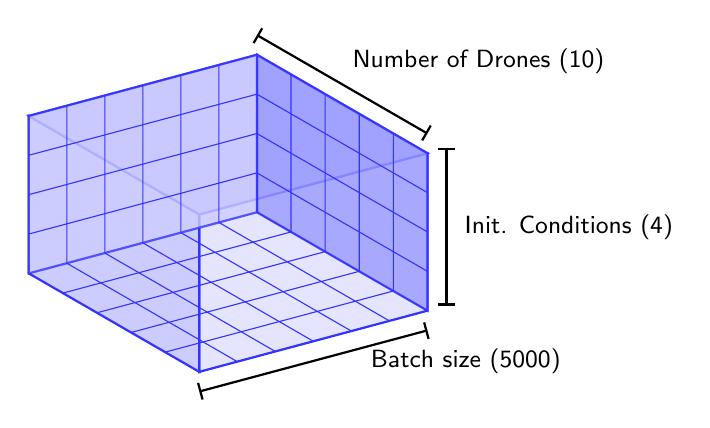
\begin{tikzpicture}[
    x=(15:0.5cm), y=(90:0.5cm), z=(330:0.5cm),
    font=\sffamily\small
]

% Dimensions
\def\pop{6}
\def\env{4}
\def\drones{5}

% Draw back faces
\fill[blue!10, draw=blue!80, thick] (0,0,\drones) -- (\pop,0,\drones) -- (\pop,\env,\drones) -- (0,\env,\drones) -- cycle;
\fill[blue!20, draw=blue!80, thick] (0,0,0) -- (0,\env,0) -- (0,\env,\drones) -- (0,0,\drones) -- cycle;

% Draw front/top/right faces (The Tensor)
\fill[blue!30, draw=blue!80, thick, opacity=0.8] (0,\env,0) -- (\pop,\env,0) -- (\pop,\env,\drones) -- (0,\env,\drones) -- cycle;
\fill[blue!40, draw=blue!80, thick, opacity=0.8] (\pop,0,0) -- (\pop,\env,0) -- (\pop,\env,\drones) -- (\pop,0,\drones) -- cycle;
\fill[blue!20, draw=blue!80, thick, opacity=0.8] (0,0,0) -- (\pop,0,0) -- (\pop,\env,0) -- (0,\env,0) -- cycle;

% Grid lines on the visible faces
\foreach \x in {1,...,\pop} {
    \draw[blue!80] (\x,\env,0) -- (\x,0,0) -- (\x,0,\drones);
}
\foreach \y in {1,...,\env} {
    \draw[blue!80] (0,\y,0) -- (\pop,\y,0) -- (\pop,\y,\drones);
}
\foreach \z in {1,...,\drones} {
    \draw[blue!80] (\pop,\env,\z) -- (\pop,0,\z) -- (0,0,\z);
}

% Labels
% Pop size label on the bottom arrete
\draw[thick, |-|] (0,-0.5,\drones) -- (\pop,-0.5,\drones) node[midway, below=0.4cm, right=0.6cm] {Batch size (5000)};

% Init conditions on the right arrete
\draw[thick, |-|] (\pop+0.5,0,\drones) -- (\pop+0.5,\env,\drones) node[midway, right=0.1cm] {Init. Conditions (4)};

% Number of drones on the top arrete
\draw[thick, |-|] (\pop,\env+0.5,0) -- (\pop,\env+0.5,\drones) node[midway, above right] {Number of Drones (10)};

\end{tikzpicture}
\caption{3D Tensor structure used for parallel swarm evaluation in PyTorch.}
\label{fig:tensorization}
\end{figure}

During the evaluation phase, each genome dictates the behavior of a simulated drone swarm over a fixed number of integration steps. The fitness of each individual is evaluated using a composite cost function that aggregates multiple behavioral metrics into a single score (see Section~\ref{sec:milling}). This function penalizes undesirable flight characteristics---such as excessive turning efforts or inter-drone collisions---while rewarding overarching mission objectives like spatial coverage or collective alignment. By blending these diverse and sometimes conflicting factors, the cost function establishes a complex fitness landscape.

To ensure the resulting swarm behaviors are robust and not merely overfitted to a specific starting layout, the algorithm evaluates each genome across multiple distinct initial spatial conditions. The framework can then assign a final fitness score using one of three evaluation strategies: ``average'', ``best'', or ``minmax''. The ``average'' strategy computes the mean cost across all environments, promoting generally good behavior but potentially masking edge-case failures. The ``best'' strategy isolates the minimum cost achieved, rewarding peak performance but risking fragility in non-ideal scenarios. Conversely, the implemented ``minmax'' strategy records the costs from all starting conditions and assigns the maximum---or worst---cost as the genome's definitive score. By actively optimizing for this worst-case scenario, the algorithm forces the selection of universally resilient configurations, significantly narrowing the reality gap for potential real-world deployment.

Following evaluation, the algorithm applies evolutionary operators to generate the next iteration of parameters. It utilizes a tournament selection mechanism with a tournament size of 3 to choose parent genomes, randomly pitting three individuals against each other and selecting the one with the lowest worst-case cost. A uniform crossover operator then blends the genes of these selected parents. To maintain genetic diversity and prevent premature convergence, a double mutation strategy is applied. First, a local mutation introduces a Gaussian scaling noise ($X \sim \mathcal{N}(1.0, 0.3^2)$), with a mutation probability $p_m(g)$ that decays as generations ($g$) progress. This allows for broad parameter search initially and fine-tuning in later stages:
\begin{equation}
    p_m(g) = 0.35 - 0.20 \left( \frac{g}{G} \right)
\end{equation}
Second, a global mutation operator introduces a large parameter jump that completely replaces genes with new random values, applied with a fixed probability of 5\% across the entire generation. This ensures the population can abruptly escape local minima in the complex, non-linear fitness landscape. Finally, a strict elitism mechanism is enforced: the single absolute best-performing parameter set is preserved entirely untouched and injected directly into the first slot of the subsequent generation, securing monotonic optimization progress throughout the training cycle.

% ---------------------------------------------------------
\section{Emergence of Collective Behaviors: Milling}
\label{sec:milling}

\subsection{Defining the Cost Function}
To actively search for specific topological phases, the fitness function evaluated by the Genetic Algorithm must explicitly reward desired macroscopic states while penalizing collisions and excessive energy consumption. We define a multi-objective cost function balancing group polarization, milling momentum, and control effort. 

\begin{itemize}
	\begin{multicols}{2}
		\item $N$: number of drones
		\item $p_i = (x_i, y_i)$: position
		\item $\phi_i$: heading
		\item $v_i$: speed
	\end{multicols}
\end{itemize}


The cost of the effort cost $c_{\text{effort}}$ is calculated as follows:

\begin{equation}
	c_{\text{effort}} = \sum_{i = 1}^{N} |\dot{\phi_i} |
\end{equation}

The center of the swarm $B$ is determined:
\begin{equation}
	B = \frac{1}{N} \sum_{i=1}^{N} p_i \\
\end{equation}

The distance of each drone to this center is calculated as such:
\begin{equation}
	d_i = \| p_i - B \|_2
\end{equation}

The cost of the dispersion cost $c_{\text{disp}}$ is calculated as follows:
\begin{equation}
	c_{\text{disp}} =  \left| \left( \frac{1}{N} \sum_{i=1}^{N} d_i \right) - 5.0 \right|
\end{equation}

The polarisation parameter is determined as follows:
\begin{equation}
	P = \sqrt{\left( \frac{1}{N} \sum_{i=1}^{N} \cos \phi_i \right)^2 + \left( \frac{1}{N} \sum_{i=1}^{N} \sin \phi_i \right)^2}
\end{equation}

This allows for the calculation of the polarisation cost $c_{\text{pol}}$:
\begin{equation}
	c_{\text{pol}} = (1 - P)
\end{equation}

To calculate the collision cost $c_{\text{coll}}$, we first determine the distance between drones:
\begin{equation}
	d_{ij} = \| p_i - p_j \|_2
\end{equation}

Thus:
\begin{equation}
	c_{\text{coll}} = \frac{1}{2} \sum_{i=1}^{N} \sum_{\substack{j=1 \\ j \neq i}}^{N} \mathbbm{1}_{(d_{ij} < d_{\text{coll}})}
\end{equation}

To compute the milling cost $c_{\text{mill}}$, we first compute the speed vector $V_i$ for each drone:
\begin{equation}
	V_i = \begin{pmatrix} v_i \cos \phi_i \\ v_i \sin \phi_i \end{pmatrix}
\end{equation}

Then we determine the average speed of the swarm:
\begin{equation}
	\bar{V} = \frac{1}{N} \sum_{i=1}^{N} V_i
\end{equation}

Thus follows the centred speed:
\begin{equation}
\Delta v_i = v_i - \bar{V}
\end{equation}

And the centred position:
\begin{equation}
\Delta p_i = p_i - B
\end{equation}

These are used to determine the angle of the postion to the swarm's centre:
\begin{equation}
	\theta_i = \text{atan2}(\Delta p_{i, y}, \Delta p_{i, x})
\end{equation}

And the angle of the speed vector to the swarm's centre:
\begin{equation}
\phi_{v, i} = \text{atan2}(\Delta v_{i, y}, \Delta v_{i, x})
\end{equation}

These then allow for the computation of the milling cost:
\begin{equation}
	c_{\text{mill}} = \left| \frac{1}{N} \sum_{i=1}^{N} \sin(\theta_i - \phi_{v, i}) \right|
\end{equation}

To ensure the stability of the emergent milling phases and prevent the swarm from drifting—a behavior frequently observed during the optimization of unconstrained circular motion—we introduce a stationary cost $c_{\text{stationary}}$. This cost penalizes the velocity of the swarm's barycenter:
\begin{equation}
	c_{\text{stationary}} = \|\bar{V}\|_2
\end{equation}

The final cost $c_{\text{tot}}$ function is the sum of all of these costs, to which the exploration cost can be added if relevant (this cost will be detailed in a further section). Each cost $c_x$ is associated to a weight $W_x$ which is used to tune the relative influences of these parameters in the final cost function:
\begin{align}
	c_{\text{tot}} &= c_{\text{effort}} \times W_{\text{effort}} \nonumber \\
	&\quad + c_{\text{disp}} \times W_{\text{disp}} \nonumber \\
	&\quad + c_{\text{pol}} \times W_{\text{pol}} \nonumber \\
	&\quad + c_{\text{coll}} \times W_{\text{coll}} \nonumber \\
	&\quad + c_{\text{mill}} \times W_{\text{mill}} \nonumber \\
	&\quad + c_{\text{stationary}} \times W_{\text{stationary}} \nonumber \\
	&\quad + c_{\text{explo}} \times W_{\text{explo}}
\end{align}


With only a pure milling weight on the cost function, by minimizing $c_{\text{tot}}$, the Genetic Algorithm successfully identified regions in the parameter space that organically lead to a stable milling formation. Figure \ref{fig:milling_success} illustrates a typical simulation output where the swarm converges into a continuous vortex, demonstrating the efficacy of our multi-objective cost function in isolating this specific topological phase.

\begin{figure}[htbp]
	\centering
	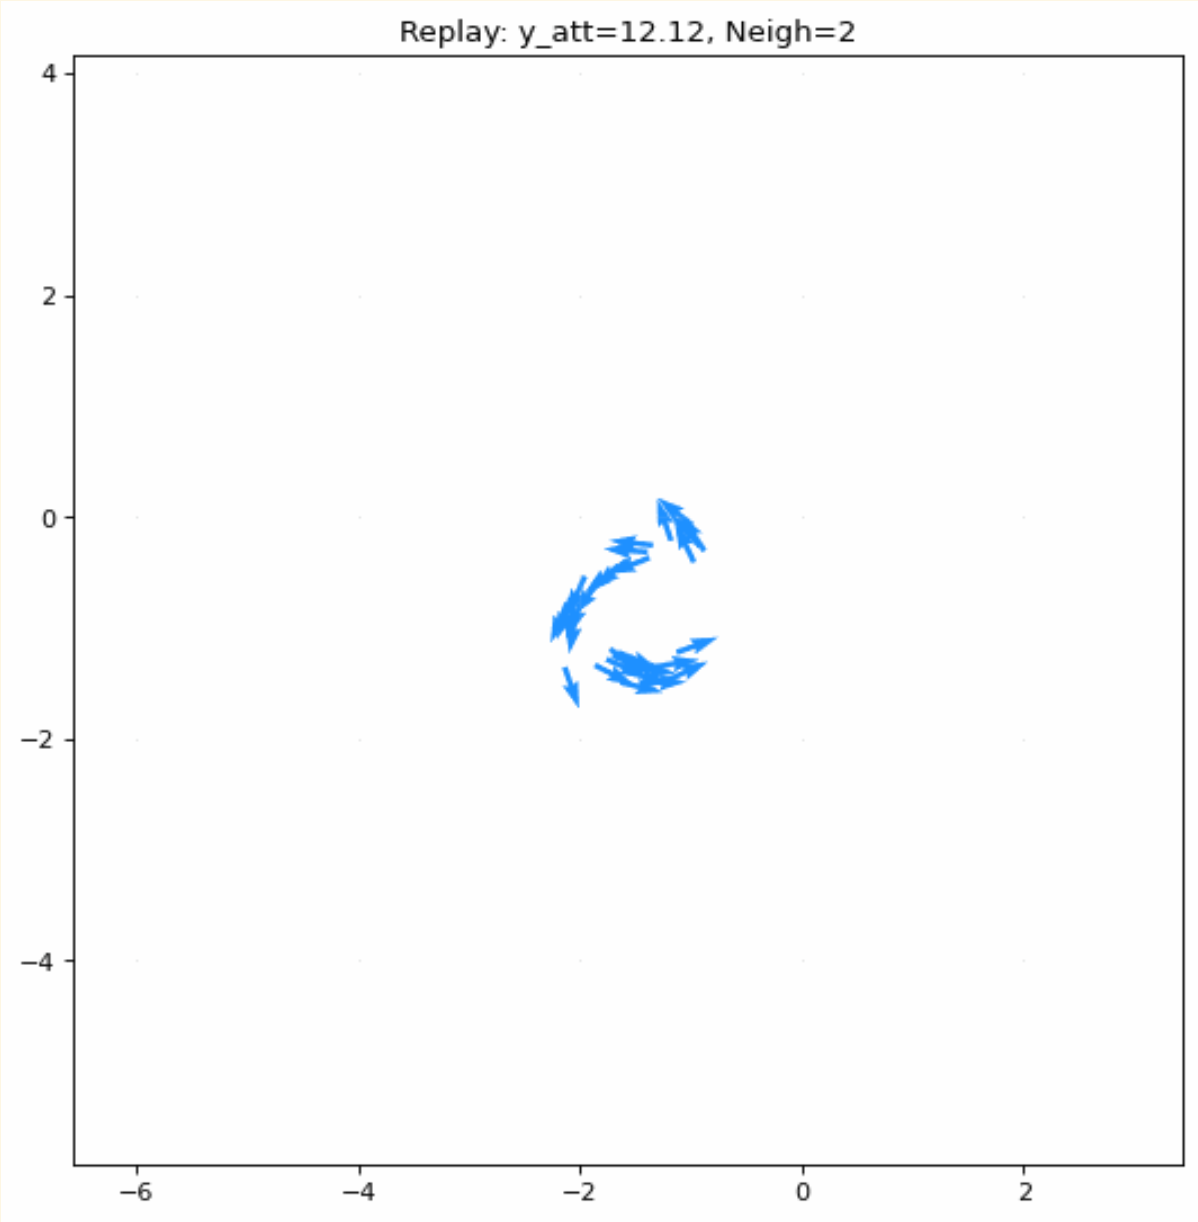
\includegraphics[width=0.85\linewidth]{milling_successful.png}
	\caption{Visual representation of a successful milling phase emerged from the GA optimization. The drones (blue vectors) exhibit stable circular motion around the swarm's barycenter while maintaining strict collision avoidance constraints.}
	\label{fig:milling_success}
\end{figure}

\subsection{Parameter Sweep and Scalability}

The emergence of a stable milling phase is notoriously difficult to achieve through manual tuning due to the highly non-linear dynamics and cascading interactions between the bio-inspired control parameters. Therefore, successfully isolating the parameter manifold that consistently triggers milling serves as a fundamental proof of concept for our Genetic Algorithm (GA). It demonstrates the algorithm's capability to navigate a complex, multi-dimensional continuous search space to optimize macroscopic swarm behaviour before applying it to more complex operational scenarios.

We initially employed the GA to discover parameter bounds that reliably trigger the milling phase for a fixed population. However, a set of parameters optimized for $N=10$ drones may degrade, shear, or cause the vortex to collapse entirely when applied to $N=30$. To ensure the robustness of our model, we conducted a systematic parameter sweep across varying swarm sizes ($N \in \{10, 15, 20, 25, 30\}$) to analyze the scalability of the discovered behavioral regions. To avoid statistical bias from generational cloning, only the absolute best, unique individual from each optimization run was extracted for analysis.

\begin{figure}[htbp]
	\centering
	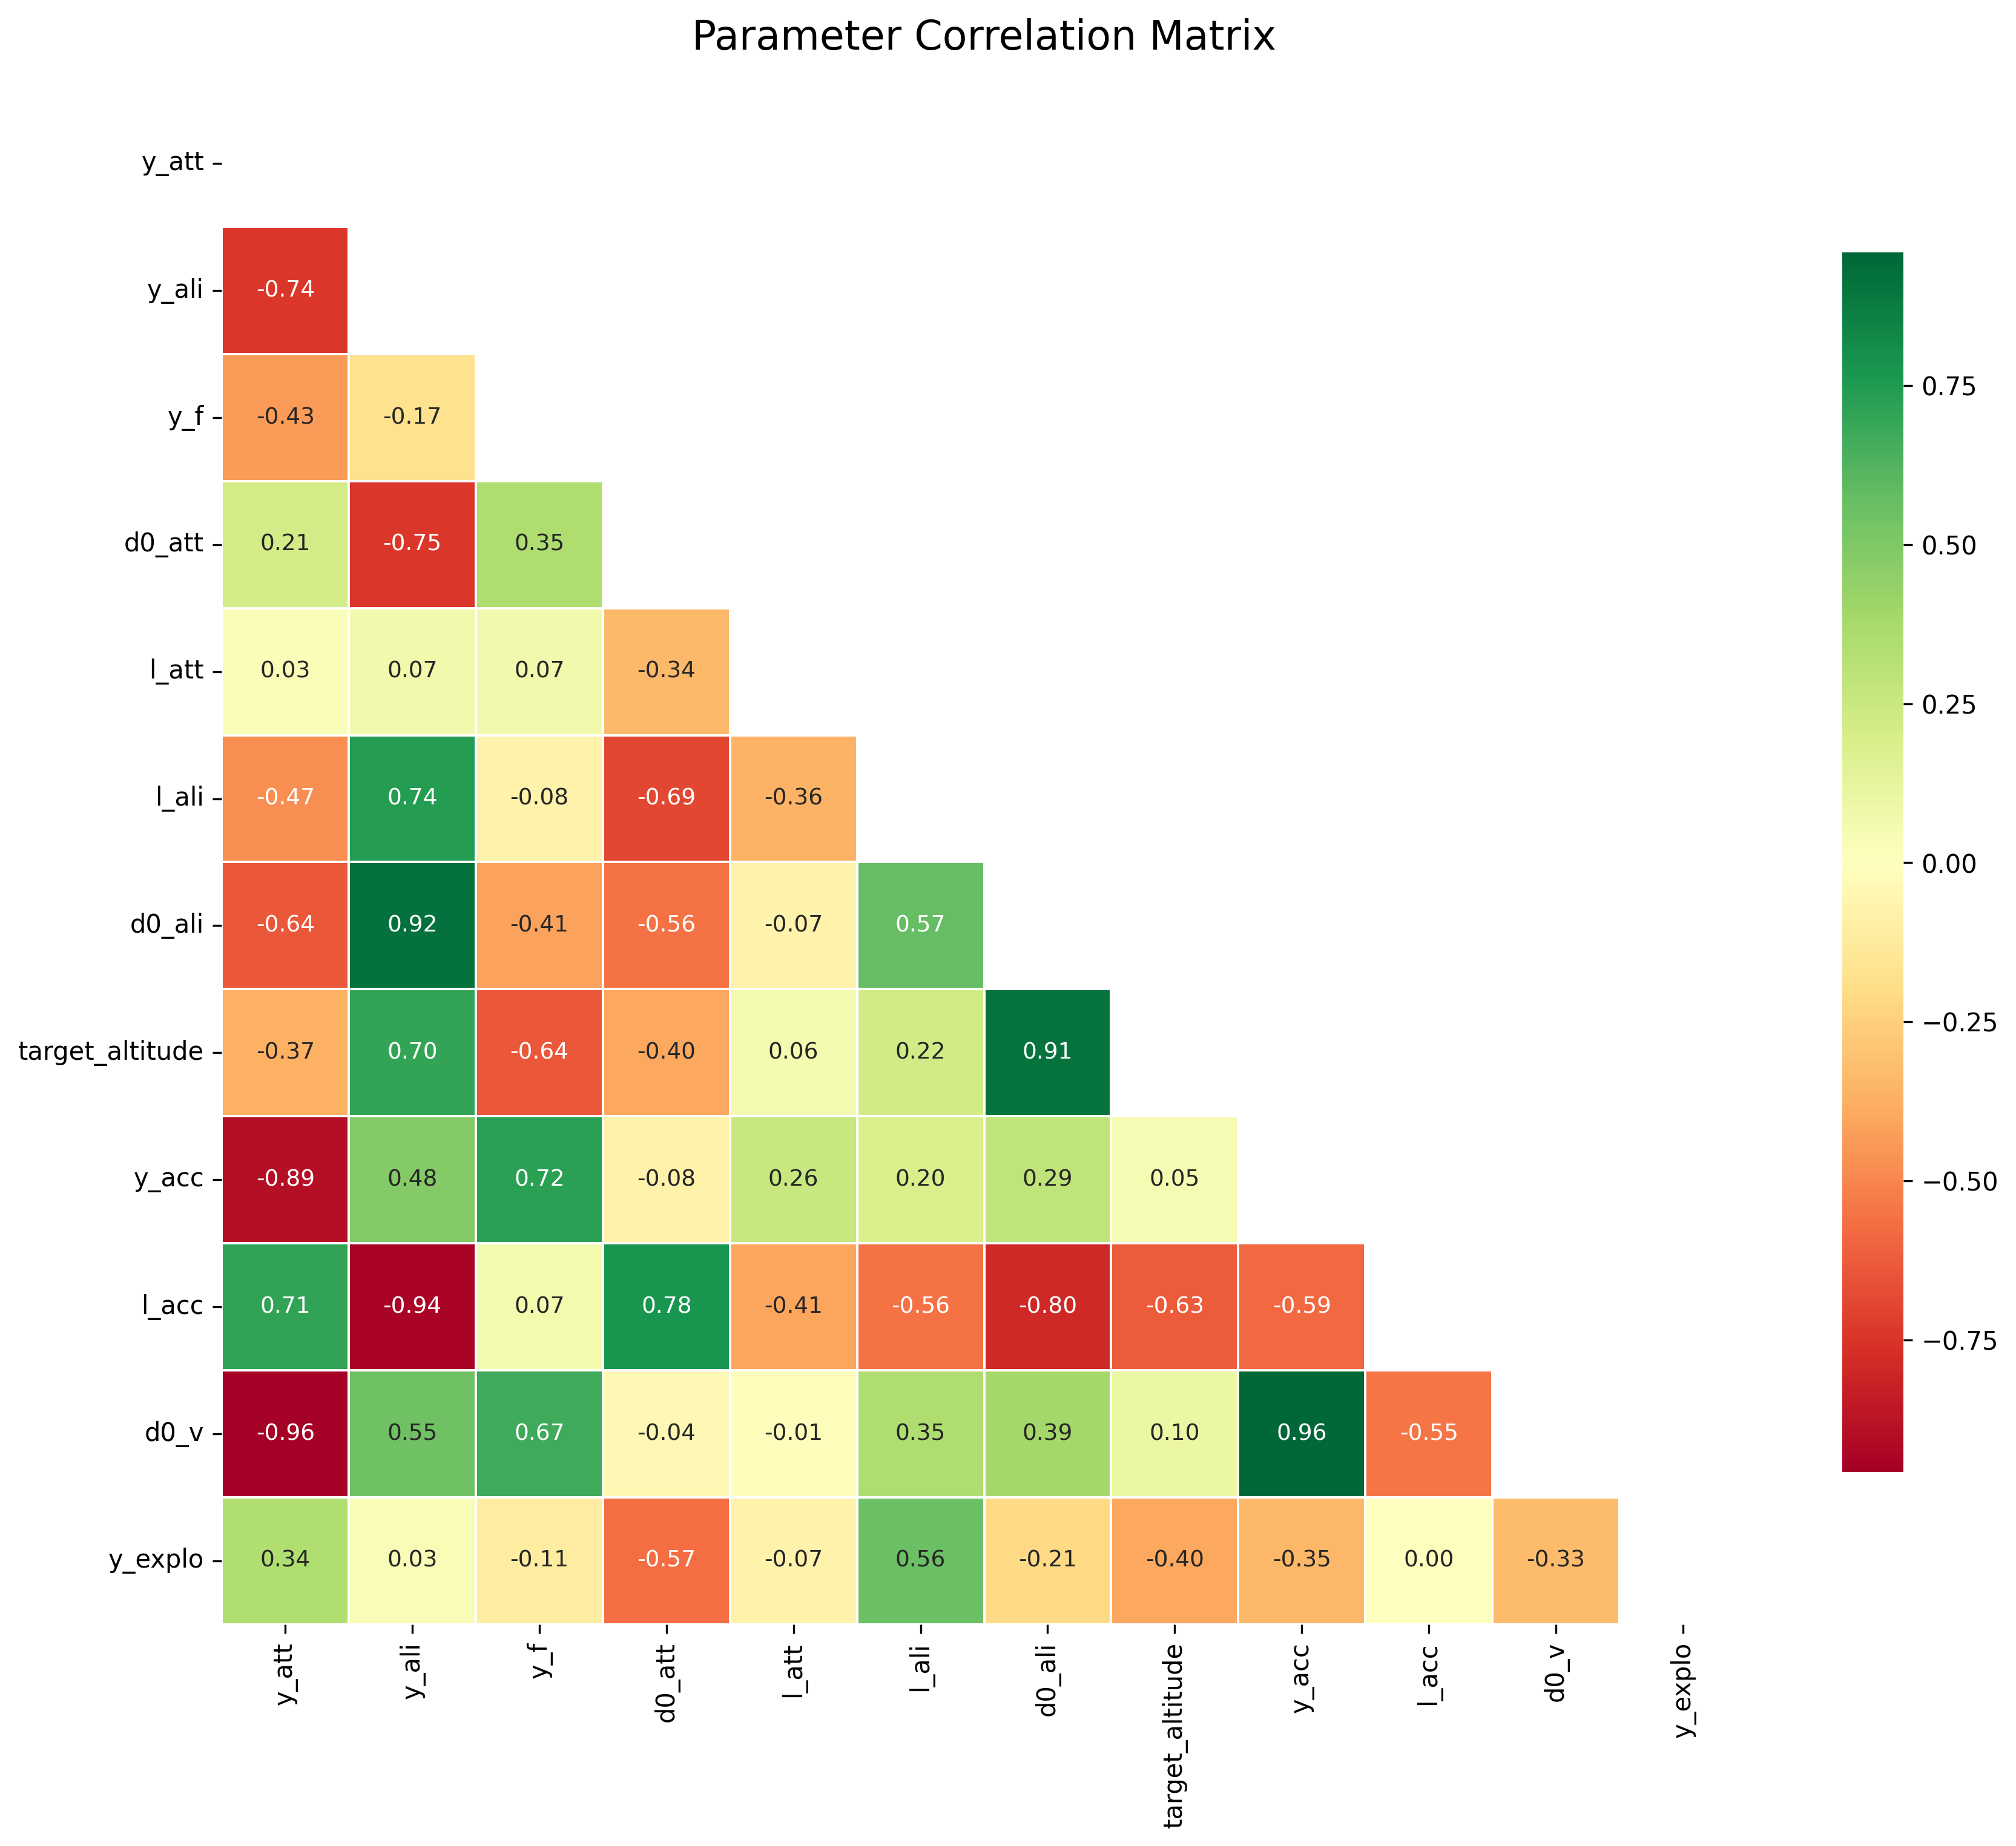
\includegraphics[width=\linewidth]{corr_matrix_2026-05-14_14-21-28.png}
	\caption{Parameter correlation matrix generated from the unique global optimums across all tested swarm sizes ($N=10$ to $30$). The diverging color scale highlights the true macroscopic scaling laws and physical trade-offs required to sustain the milling phase at any scale.}
	\label{fig:correlation}
\end{figure}

The resulting correlation matrix (Fig. \ref{fig:correlation}) filters the dataset to include only the active genes, revealing the underlying physical rules the GA had to discover to maintain the vortex formation at scale. The matrix highlights three critical dynamic dependencies:

\begin{itemize}
	\item \textbf{Kinematic Synchronization Scaling ($r = 0.96$):} A near-perfect positive correlation exists between the social acceleration multiplier ($y_{\text{acc}}$) and the nominal velocity distance ($d0_{\text{v}}$). The algorithm discovered a fundamental scaling law for speed synchronization: as the swarm's scale changes, a larger zone of speed influence must be compensated by a proportionally stronger acceleration authority. This ensures that agents on the outer edge of a larger milling ring can accelerate rapidly enough to keep pace with the inner agents.
	
	\item \textbf{Alignment Field Proportionality ($r = 0.92$):} The matrix shows a very strong positive correlation between the alignment strength ($y_{\text{ali}}$) and the core alignment distance ($d0_{\text{ali}}$). If the GA selects a high gain for heading alignment, it must simultaneously widen the geometric zone where this force applies, preventing high-frequency heading oscillations that would destroy the smooth circular flow.
	
	\item \textbf{The Heading vs. Velocity Priority Trade-off ($r = -0.94$):} There is a severe negative correlation between the acceleration length scale ($l_{\text{acc}}$) and the alignment strength ($y_{\text{ali}}$). The GA identified that the swarm cannot rely heavily on both heading alignment and distant velocity synchronization simultaneously. If the swarm prioritizes matching headings, it must restrict the radius of speed adjustments to prevent conflicting command inputs that could fracture the swarm.
\end{itemize}

Ultimately, this parameter sweep demonstrates that the scalability of the bio-inspired swarm does not rely on a single, rigid set of parameters, but rather on a multidimensional manifold of ratios. By identifying these strict relational constraints, the genetic programming approach validated its efficiency in optimizing distributed flight dynamics.

% ---------------------------------------------------------
\section{Application to Exploration and SAR Scenarios}
\label{sec:exploration}

\subsection{The Grid Coverage Problem}
In Search and Rescue (SAR) operations, the primary objective translates mathematically to an area coverage optimization problem. The operational space is discretized into a 2D grid. The swarm's performance is intrinsically linked to its ability to explore the grid completely. Another important aspect of SAR scenarios is that the target might not stay in the same place during the whole scenario. This means that drones must overfly each cell of the grid repeatedly to ensure they extract as much information as possible from the environment.

\begin{figure}[htbp]
	\centering
	% \rule{\linewidth}{4.5cm}
	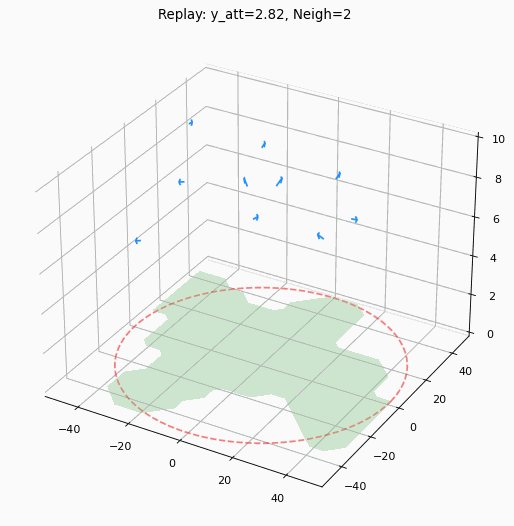
\includegraphics[width=0.85\linewidth]{explo_visualisation.png}
	\caption{Heatmap demonstrating the spatial coverage of the drone swarm operating under GA-optimized parameters.}
	\label{fig:heatmap}
\end{figure}

\subsection{Fitness Evaluation for Exploration}
The exploration fitness relies on two main factors: the continuous discovery of unseen areas and the periodic revisiting of previously explored zones. This mimics the decay of information relevant in dynamic SAR environments. The amount of information known about the cell is described by a numerical value called freshness. At the beginning of the scenario, each cell has a minimal freshness. As drones traverse the environment, they increase the freshness of the cells they overfly. To represent the information going stale over time, the freshness decreases (at first slowly, then faster as time passes).

The quality of the information gathered from a flight at low altitude is naturally better than that of the information gathered from a high altitude flight. However flying at higher altitude means the camera can see a wider area and thus gather more information. This relationship is taken into account by the fitness calculation. Each drone can "see" in a cone below them. If they fly high, they increase the freshness of a large amount of cells by a small amount. If they fly lower, they increase the freshness of a few cell by a larger amount.

The coverage of the grid is measured by counting the number of cells which are deemed "explored". For this to be the case the cell's freshness must exceed \SI{10}{\%} of the maximum freshness value. The coverage is then normalised by the total amount of cells in the grid. In the case where each drone has its own map of the grid (see section \ref{sec:information}), a global grid is constructed with the best freshness found a cross the individual grids. This global grid is then used to calculate the coverage. The exploration cost $c_{\text{explo}}$ is this measure of the grid's coverage.

% ---------------------------------------------------------
\section{Distributed Information Gathering Strategies}
\label{sec:information}

A genetic algorithm can only be as good as its fitness function. In the case of a SAR scenario the fitness depends a lot on how the gathered information is shared between the drones in the swarm.

\subsection{Pheromone-based Stigmergic Coordination}
One such method is pheromone-based stigmergic coordination \cite{devaraju_connectivity-aware_2023, xuan_dual-trail_2026}. This method relies on digital pheromones being released by the drones to mark the cells they have explored. These pheromones decay and disappear over time, representing the information losing relevance as time goes on. The pheromones repel other drones, thus encouraging the swarm to fly to cells which have yet to be explored.

Xuan et al. \cite{xuan_dual-trail_2026} have even explored how the use of two distinct pheromones in an exploration scenario: a short term pheromone to encode the recent activity of the swarm and a long term pheromone to encode the global exploration coverage. They have showed this method can achieve a very high coverage uniformity of the water column.

In our simulation model, this stigmergic coordination is mathematically inverted and implemented through a discrete spatial ``spoilage grid''. Instead of maximizing freshness, the grid tracks spoilage, starting at a maximum value $S_{max}$ representing completely unexplored territory. As agents traverse the environment, they clear this spoilage. To account for altitude and sensor mechanics, the update is not a simple cell overwrite but a 2D Gaussian splat governed by the Inverse Square Law. The intensity and spread of the clearing effect dynamically depend on the drone's altitude ($Z$) and its Field of View (FOV). 

To simulate the decaying relevance of information over time, the grid undergoes a uniform time-step spoilage accumulation governed by a multiplicative factor $\mu_{spoil}$ and an additive factor $\alpha_{spoil}$:
$$S_{t+1}(x,y) = \min(S_{max}, S_t(x,y) \cdot \mu_{spoil} + \alpha_{spoil})$$
This increasing spoilage acts as an attractive virtual pheromone. Agents compute an exploration gradient vector directing them towards high-spoilage areas, driving the swarm naturally to continuously revisit and explore regions.

\subsection{Impact of Communication Topologies}
To evaluate the sim-to-real gap regarding network constraints, we compare several information-sharing topologies. The exploration framework relies on two distinct but complementary mechanisms: the map storage and sharing strategy (\texttt{MAP\_STRATEGY}), and the navigation decision-making (\texttt{EXPLO\_STRATEGY}).

While a centralized oracle provides theoretical maximum efficiency by granting all agents instantaneous access to a master freshness grid, real-world UAVs rely on distributed mesh networks with limited bandwidth and range. To accurately model these constraints, we implemented and evaluated three distinct communication paradigms for map synchronization:

\begin{itemize}
	\item \textbf{Global Oracle (\texttt{global}):} Agents have perfect, real-time knowledge of the entire environment's map. Every drone updates and reads from a single, centralized tensor. This serves as our theoretical upper-bound baseline.
	
	\vspace{0.2cm}
	\begin{center}
		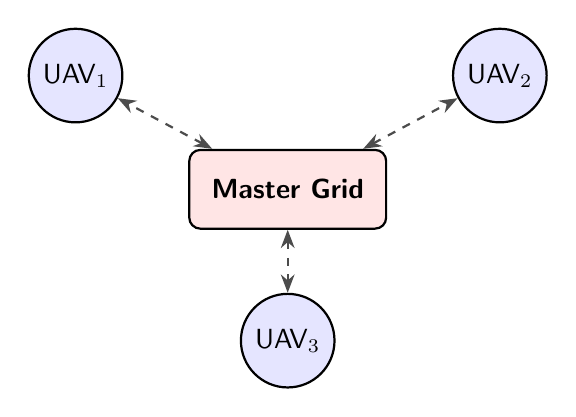
\begin{tikzpicture}[
			drone/.style={circle, draw=black, fill=blue!10, thick, minimum size=0.8cm, font=\sffamily},
			oracle/.style={rectangle, draw=black, fill=red!10, thick, rounded corners, minimum width=2.5cm, minimum height=1cm, font=\bfseries\sffamily},
			comm/.style={<->, >=Stealth, thick, dashed, draw=black!70}
			]
			\node[oracle] (master) {Master Grid};
			\node[drone] (d1) [above left=0.5cm and 1cm of master] {UAV$_1$};
			\node[drone] (d2) [above right=0.5cm and 1cm of master] {UAV$_2$};
			\node[drone] (d3) [below=0.8cm of master] {UAV$_3$};
			
			\draw[comm] (master) -- (d1);
			\draw[comm] (master) -- (d2);
			\draw[comm] (master) -- (d3);
		\end{tikzpicture}
	\end{center}
	\vspace{0.2cm}
	
	\item \textbf{Local Shared Map (\texttt{local\_shared}):} Agents maintain individual, localized versions of the map. Synchronization occurs between drones using a topological approach rather than a strictly spatial one. Specifically, map data is shared unilaterally with an agent's $K$-Nearest Neighbors (e.g., $K=2$). Furthermore, to simulate bandwidth constraints, this map synchronization is not continuous but occurs at a discrete interval of $\tau_{sync}$ ticks (e.g., \texttt{REFRESH\_MAP\_TICKS} $= 50$).
	
	\vspace{0.2cm}
	\begin{center}
		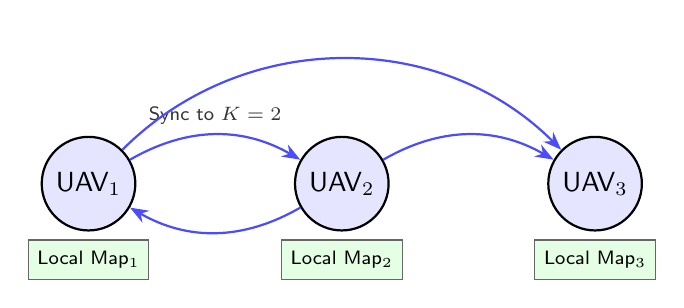
\begin{tikzpicture}[
			node distance=2cm,
			drone/.style={circle, draw=black, fill=blue!10, thick, minimum size=0.8cm, font=\sffamily},
			map/.style={rectangle, draw=black!60, fill=green!10, minimum width=1.2cm, minimum height=0.5cm, font=\scriptsize\sffamily},
			comm/.style={->, >=Stealth, thick, draw=blue!70}
			]
			\node[drone] (d1) {UAV$_1$};
			\node[map] (m1) [below=0.1cm of d1] {Local Map$_1$};
			
			\node[drone] (d2) [right=of d1] {UAV$_2$};
			\node[map] (m2) [below=0.1cm of d2] {Local Map$_2$};
			
			\node[drone] (d3) [right=of d2] {UAV$_3$};
			\node[map] (m3) [below=0.1cm of d3] {Local Map$_3$};
			
			% D1 sharing to K=2 neighbors
			\draw[comm] (d1) to[bend left=30] node[midway, above, font=\scriptsize\sffamily, text=black!80] {Sync to $K=2$} (d2);
			\draw[comm] (d1) to[bend left=45] (d3);
			
			% D2 sharing to K=2 neighbors
			\draw[comm] (d2) to[bend left=30] (d1);
			\draw[comm] (d2) to[bend left=30] (d3);
		\end{tikzpicture}
	\end{center}
	\vspace{0.2cm}
	
	\item \textbf{Local Individual Map (\texttt{local\_individual}):} To severely reduce communication overhead and eliminate structural dependencies, drones do not exchange any map data over the network. Instead, each drone relies strictly on its own isolated memory grid, which is updated solely by its own field of view (FOV).
	
	\vspace{0.2cm}
	\begin{center}
		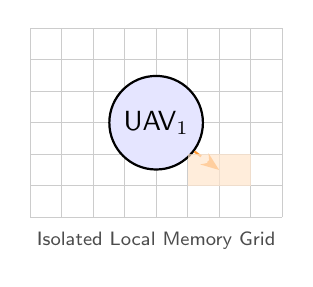
\begin{tikzpicture}[
			drone/.style={circle, draw=black, fill=blue!10, thick, minimum size=0.8cm, font=\sffamily},
			gridline/.style={draw=black!20, thin},
			sensor/.style={->, >=Stealth, thick, draw=orange!80, dashed}
			]
			% Local grid background
			\draw[gridline, step=0.4cm] (-1.6,-1.2) grid (1.6,1.2);
			
			\node[drone] (d1) at (0,0) {UAV$_1$};
			
			% Sensor updating local map only
			\draw[sensor] (d1) -- (0.8, -0.6) node[midway, below left, text=orange!80, font=\scriptsize\sffamily] {};
			\fill[orange!20, opacity=0.7] (0.4, -0.8) rectangle (1.2, -0.4);
			
			\node[font=\scriptsize\sffamily, text=black!70] at (0, -1.5) {Isolated Local Memory Grid};
		\end{tikzpicture}
	\end{center}
	\vspace{0.2cm}
\end{itemize}

\subsection{Experimental Results and Comparative Analysis}
To evaluate these topologies, we conducted a systematic parameter sweep crossing the mapping strategies with two decision policies: \texttt{local\_gradient} (gradient descent on spoilage) and \texttt{global\_best} (greedy targeting of the absolute maximum). The cost function minimizes $C_{total}$ with weights $W_{\text{coll}} = 500$ (collision penalty) and $W_{\text{explo}} = -50$ (coverage reward).

\begin{table}[htbp]
	\caption{Performance metrics across communication and decision strategies.}
	\label{tab:results}
	\centering
	\begin{tabular}{llcc}
		\toprule
		\textbf{Map Strategy} & \textbf{Decision Policy} & \textbf{Total Cost} $\downarrow$ & \textbf{Coverage (\%)} $\uparrow$ \\ 
		\midrule
		\texttt{global} & \texttt{global\_best} & \textbf{-134,454} & 89.56\% \\
		\texttt{global} & \texttt{local\_gradient} & -133,718 & 91.14\% \\
		\texttt{local\_shared} & \texttt{global\_best} & -130,901 & 87.97\% \\
		\texttt{local\_shared} & \texttt{local\_gradient} & -127,638 & 89.56\% \\
		\texttt{local\_individual} & \texttt{global\_best} & -121,514 & \textbf{93.35\%} \\
		\texttt{local\_individual} & \texttt{local\_gradient} & -120,901 & 71.52\% \\ 
		\bottomrule
	\end{tabular}
\end{table}

\begin{figure}[htbp]
	\centering
	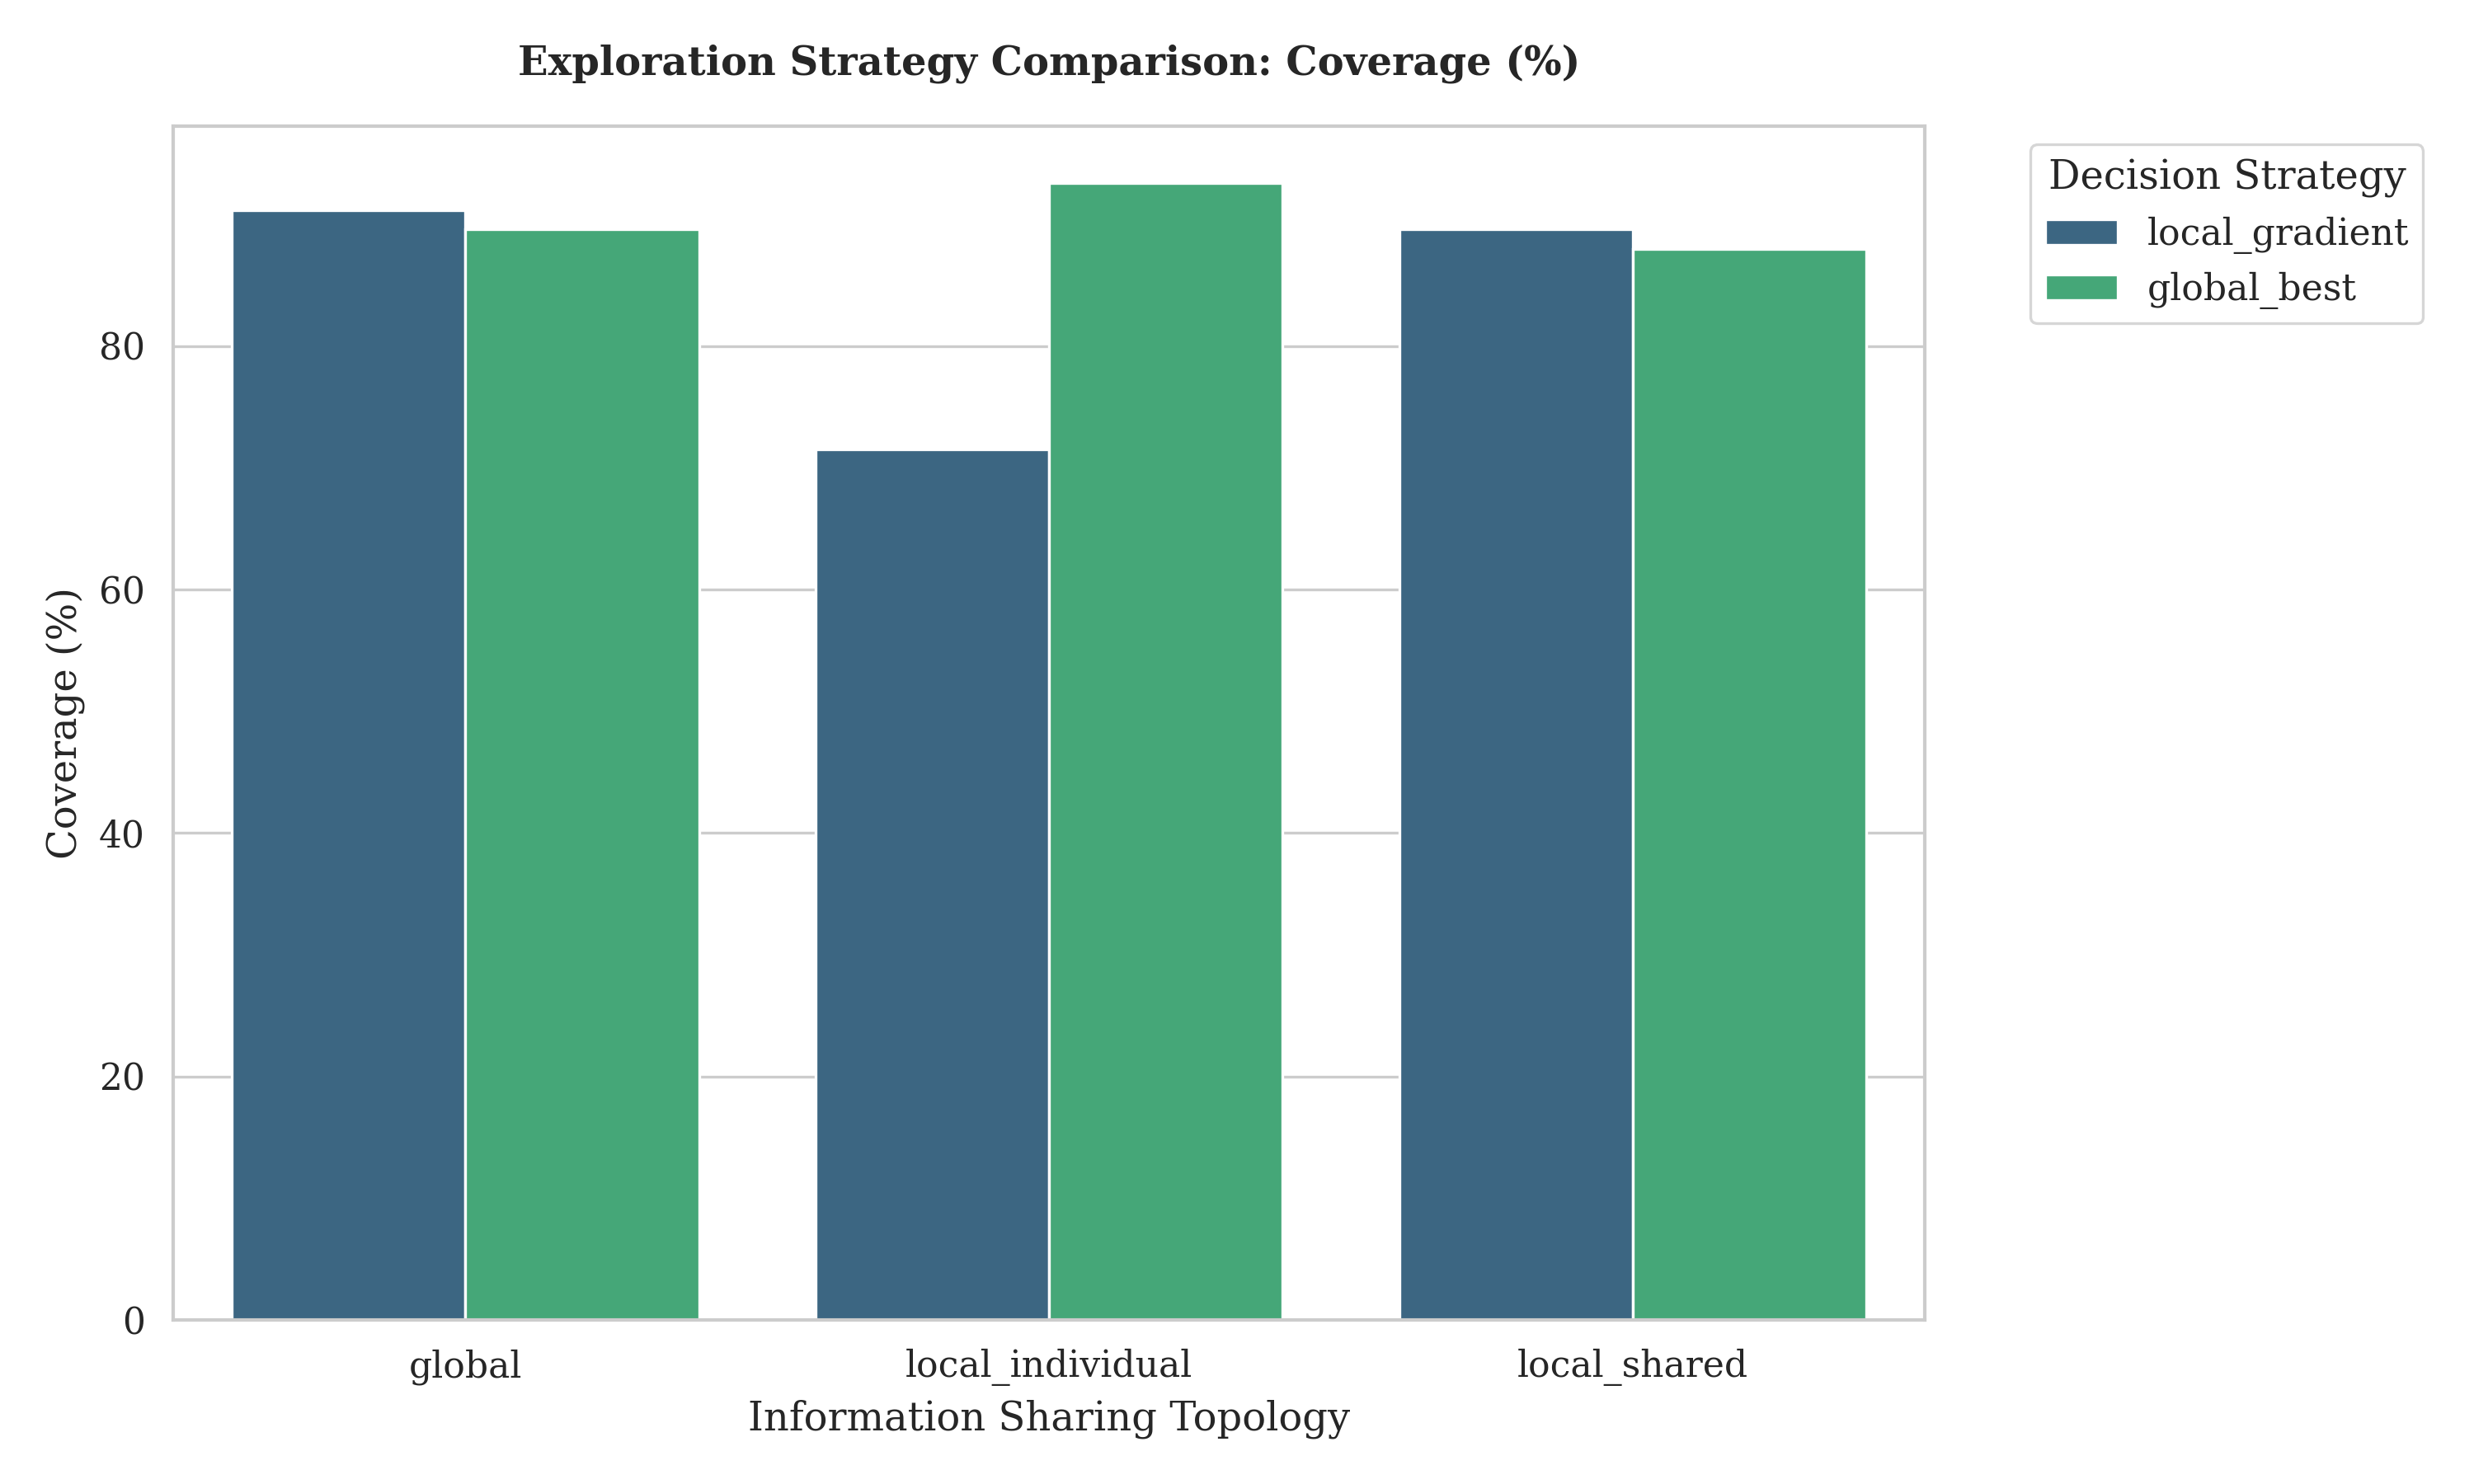
\includegraphics[width=0.9\linewidth]{bar_comparison_Coverage_(pct).png}
	\caption{Comparison of area coverage across topologies. Distributed sharing (\texttt{local\_shared}) maintains efficiency close to the global oracle despite bandwidth constraints.}
	\label{fig:coverage_results}
\end{figure}

\subsubsection{Analysis of the Isolation Paradox}
The results in Table~\ref{tab:results} reveal that the highest raw coverage (\textbf{93.35\%}) is achieved in total isolation (\texttt{local\_individual}). However, this configuration yields the worst global cost (-121,514). Without communication, drones target global maxima independently, leading to a "chaotic explosion" of the swarm. While this covers more area, the lack of coordination causes frequent trajectory intersections. Given that $W_{\text{coll}}$ is ten times higher than $W_{\text{explo}}$, the resulting collision penalties negate the exploration gains.

\subsubsection{Network Resilience and Bio-inspired Fluidity}
The \texttt{local\_shared} topology achieves \textbf{89.56\%} coverage, performing remarkably close to the global oracle. Coupled with \texttt{local\_gradient}, the swarm maintains a fluid, ameba-like motion that minimizes collision risks. This validates that asynchronous, low-bandwidth sharing of localized maps is sufficient to successfully propagate stigmergic information and maintain efficient Search and Rescue operations in network-constrained environments. Indeed, comparable performance is achieved between the two map-sharing configurations, despite the distributed approach requiring less than a tenth of the network bandwidth

% ---------------------------------------------------------
\section{Discussion and Conclusion}
\label{sec:conclusion}

The optimization of bio-inspired swarm parameters through genetic programming presents significant advantages for tailoring complex multi-agent systems to specific operational requirements. By leveraging PyTorch tensor operations, our framework massively parallelized the simulation environments, enabling the rapid and simultaneous evaluation of thousands of swarm configurations. Through the optimization of a multi-objective fitness function, the Genetic Algorithm successfully isolated parameter combinations that balance robust milling behavior, efficient area coverage, and minimal control effort.

A primary contribution of this study is the integration of realistic communication constraints into the evaluation pipeline. The implementation of discrete exploration modes, ranging from a centralized global oracle to decentralized local gradients and delayed map sharing, demonstrates how network limitations directly impact emergent swarm behaviors and global coverage efficiency. Furthermore, our parameter sweeping methodology highlighted the swarm's scalability challenges, quantitatively mapping how parameters optimized for a specific number of agents behave when deployed across varying swarm sizes.

Future work must focus on further narrowing the sim-to-real gap. While the current physics engine successfully incorporates inter-agent collision avoidance and basic kinematic updates, transitioning to a fully dynamic quadrotor simulation is the next critical step. This necessitates the introduction of sensory noise, complex communication packet loss models, and high-fidelity aerodynamic constraints. Additionally, integrating dynamic obstacles and individual battery life constraints will be essential to validate the robustness of these bio-inspired control algorithms for real-world Search and Rescue deployments.






% ---------------------------------------------------------
% BIBLIOGRAPHY
% ---------------------------------------------------------
\bibliographystyle{IEEEtran}
\bibliography{bibPIR}
% ---------------------------------------------------------


% ---------------------------------------------------------
\end{document}
